\chapter{多重度、熵与约束平衡}

\lectureoverview{一旦概率分布的各状态带有能量，它就成为一个热力学对象。我们首先把熵增与平衡化联系起来，并利用\(dE=T\,dS\)导出热流的方向。随后，我们将一个系统替换为大量复制品构成的大集合，对与每一组占据数相对应的排列方式进行计数，并证明这一多重度的对数等于\(N\)乘以熵。因此，平衡是一个受约束的最大熵问题。拉格朗日乘子提供了求解该问题所需的方法。}

\section{三个基本量}

设\(i\)标记系统可用的离散状态。就目前而言，离散性是有用的，因为它使我们能够在不引入相空间测度的情况下对状态进行计数。若状态\(i\)的概率为\(P_i\)，则
\begin{equation}
 \sum_i P_i=1.
 \label{eq:sm3-normalization}
\end{equation}
若该状态的能量为\(E_i\)，则平均能量为
\begin{equation}
 \overline E=\sum_iP_iE_i.
 \label{eq:sm3-mean-energy}
\end{equation}
\emph{平均}一词很重要。系统在任何单个微观状态中都不必具有值\(\overline E\)；它是各可能值按概率加权的平均值。

\begin{classroomqa}
\classquestion{这里概率与统计之间是否存在有用的区分？}
\lecturerresponse{概率为可能的结果提供模型，而统计通常从观测数据出发，追问能从中推断出什么。当前的计算使用的是概率分布，尽管同样的平均值自然会出现在统计数据中。课堂上这一非正式的交流对这两个词处理得比较随意，因为这一区分并不影响后续的物理。
\lecturetimestamp{00:01:39--00:02:21}}
\end{classroomqa}

该分布的熵为
\begin{equation}
 S[P]=-\sum_iP_i\log P_i.
 \label{eq:sm3-entropy}
\end{equation}
此表达式非负。每个非零概率都满足\(0<P_i\leq1\)，因此\(\log P_i\leq0\)，而当\(P_i\to0\)时，适用通常的极限值\(P_i\log P_i\to0\)。

\begin{figure}[t]
\centering
\includegraphics[width=0.88\textwidth]{lecture_03_figure_02.png}
\caption{开场的板书将熵、归一化和平均能量公式连同定性的一族平衡分布汇集在一起。}
\lectureframe{00:06:44}
\end{figure}

\section{作为一族分布的平衡}

上一讲给我们留下了一族单参数的平衡分布。人们可以用温度来标记这一族分布，但目前用平均能量\(\overline E\)来标记它更为有用。在最低可能能量处，分布集中在一个基态上：
\[
 P_i=\delta_{i0}.
\]
此时状态没有任何不确定性，且\(S=0\)。随着平衡分布扩展到更多能级上，其平均能量和熵都增大。

这是关于热学族分布的陈述，而不是关于一切可以设想出来的分布的陈述。任意一族分布可能在向更大能量移动的同时变得更窄。将要导出的平衡分布在通常的正温度区域内不会如此。沿着这一族分布，
\begin{equation}
 \frac{dS}{d\overline E}>0.
 \label{eq:sm3-positive-temperature-branch}
\end{equation}
具有有界谱的系统也可以有使该导数为负的分支。这些负温度区域是真实存在的，但在当前的论证中我们将其搁置一旁。

热平衡不仅仅意味着微观上的静止。分子继续运动、碰撞并交换能量。变得定常的是宏观描述：分布不再表现出净漂移，系统的各个分离部分不再维持净能量流。

\section{统计语言中的热力学定律}

第一定律是能量守恒。第二定律说，一个孤立宏观系统的热力学熵不会减少：
\begin{equation}
 \Delta S_{\mathrm{tot}}\geq0.
 \label{eq:sm3-second-law}
\end{equation}
等号描述的是平衡或理想的可逆变化；自发弛豫通常给出严格增加。

在概率图像中，弛豫倾向于将权重散布到我们仍然区分的那些宏观备选情形上。这一陈述需要讲座中强调的限定：我们是在\emph{粗粒化}。精确的哈密顿演化保持细粒化的相空间熵不变。宏观熵之所以增长，是因为我们不再追踪微观的关联和细节。丢失这类信息会拓宽约化描述。相反，自发的变窄则意味着我们在没有进行测量的情况下获得了微观信息。

第零定律断言系统能够达到热平衡，并且平衡具有传递性。如果\(A\)与\(B\)处于平衡，而\(B\)与\(C\)处于平衡，那么\(A\)与\(C\)处于平衡。温度提供了使这种传递性变得显然的数值：
\[
 T_A=T_B,\qquad T_B=T_C
 \quad\Longrightarrow\quad
 T_A=T_C.
\]
在非平衡时，能量从温度较高的子系统流向温度较低的子系统。当温度相等时，净流动停止。现在我们从温度的熵定义出发推导这一操作性陈述。

\section{为什么能量从热流向冷}

考虑两个弱耦合的子系统\(A\)和\(B\)。每个子系统内部都处于平衡，但它们的温度不同。选择标记使得
\begin{equation}
 T_B>T_A>0.
 \label{eq:sm3-temperature-order}
\end{equation}
在一次小交换过程中，组合能量的守恒给出
\begin{equation}
 dE_A+dE_B=0.
 \label{eq:sm3-energy-conservation}
\end{equation}
第二定律给出
\begin{equation}
 dS_A+dS_B\geq0.
 \label{eq:sm3-entropy-change}
\end{equation}
对于每个内部平衡的子系统，温度由下式定义
\begin{equation}
 dE_X=T_X\,dS_X,
 \qquad X=A,B.
 \label{eq:sm3-temperature-differential}
\end{equation}
代入\eqref{eq:sm3-energy-conservation}得到
\begin{equation}
 T_A\,dS_A+T_B\,dS_B=0,
\end{equation}
因而
\begin{equation}
 dS_B=-\frac{T_A}{T_B}\,dS_A.
 \label{eq:sm3-dsb}
\end{equation}
将此结果代入\eqref{eq:sm3-entropy-change}，
\begin{align}
 dS_{\mathrm{tot}}
 &=dS_A-\frac{T_A}{T_B}dS_A\\
 &=\frac{T_B-T_A}{T_B}\,dS_A\geq0.
 \label{eq:sm3-flow-entropy}
\end{align}
因为\(T_B-T_A>0\)且\(T_B>0\)，自发交换要求
\[
 dS_A>0.
\]
于是方程\eqref{eq:sm3-temperature-differential}给出
\begin{equation}
 dE_A=T_A\,dS_A>0,
 \qquad
 dE_B=-dE_A<0.
 \label{eq:sm3-hot-to-cold}
\end{equation}
能量已从\(B\)，即较热的子系统，流向\(A\)，即较冷的子系统。这里热量仅仅是传输中的能量。流动持续到\(T_A=T_B\)，此时一阶熵变不再偏向任何一个方向。

同样的结果可以写成一行：
\begin{equation}
 dS_{\mathrm{tot}}
 =dE_A\left(\frac{1}{T_A}-\frac{1}{T_B}\right)\geq0.
 \label{eq:sm3-compact-flow}
\end{equation}
逆温度差的符号决定了\(dE_A\)的符号。这种紧凑形式以后将自然地与正则系综相契合。

\begin{classroomqa}
\audiencequestion{这个论证是否假设\(A\)和\(B\)各自已经处于内部平衡？}
\lecturerresponse{是的。指定单一的\(T_A\)或\(T_B\)就作出了这一假设。如果某个子系统内部未达到平衡，就把它分成更小的区域，并在能够定义温度的每个局部应用该论证。整体的弛豫则由这些区域之间的交换组合而成。
\lecturetimestamp{00:24:38--00:25:22}}
\end{classroomqa}

\section{什么算作一个态？}

在询问平衡概率之前，我们必须知道标记\(i\)意味着什么。微观态是底层物理定律所允许的对系统的最完整描述。在经典力学中，人们设想所有粒子的位置和动量。在量子力学中，态则是一个完整的量子态；不确定性原理阻止同时精确指定每一个经典位置和动量。

对于有限盒子中的量子系统，相关的态计数可以是离散的。经典统计力学在适当的极限下出现，此时对密集分布的量子态求和变为相空间积分。这一取极限的过程还引入了使连续熵无量纲化所需的相空间元胞；它并非仅仅通过把求和号换成积分号就能得到。

\begin{classroomqa}
\audiencequestion{对于气体，是否应当把一个态想象为每个分子的位置和动量？}
\lecturerresponse{这是正确的经典图像。更一般地说，一个态意味着在物理定律约束下原则上能够知道的关于系统的一切。量子力学改变了这种最大描述的形式，并使有限体积下的计数变为离散的。从量子求和恢复经典积分是一个真正的取极限论证，而不是一行替换。
\lecturetimestamp{00:25:31--00:27:38}}
\end{classroomqa}

\section{由复制品构成的热浴}

现在无法回避这个困难的问题：在平衡建立之后，什么决定了\(P_i\)？

将子系统与一个非常大的热浴接触。能量可以来回传递，但热浴具有如此多的自由度，以至于少量能量的转移几乎不改变其温度。一种特别方便的热浴由子系统自身的许多弱耦合复制品组成。一个复制品是所研究的系统；其余复制品构成它的环境。

这种构造常常对应一个真实的宏观系统。将一个大体上近乎均匀的物体分成许多相似的元胞。每个元胞是一个子系统，而其余元胞充当它的热浴。用\(N\)表示复制品的总数。课堂演示使用九个复制品和三种有颜色的态标记，但计数与这些具体数字无关。

设\(n_i\)为处于态\(i\)的复制品数目。这些就是\emph{占据数}。可能的能级可以有无限多个，但在有限总能量下，大多数非常高的能级的占据数可以忽略或为零。

第一个约束条件就是复制品的数目：
\begin{equation}
 \sum_i n_i=N.
 \label{eq:sm3-number-constraint}
\end{equation}
第二个是总能量：
\begin{equation}
 \sum_i n_iE_i=N\overline E.
 \label{eq:sm3-total-energy-constraint}
\end{equation}
右端是广延量。若复制品的数目加倍而它们的统计状态保持不变，则总能量加倍，而每个复制品的平均能量仍为\(\overline E\)。

\begin{classroomqa}
\audiencequestion{复制品构造是否也必须满足一个能量约束？}
\lecturerresponse{是的。占据数之和必须等于\(N\)，而它们的能量加权和必须等于固定的总能量\(N\overline E\)。这正是之后将限制熵最大值的两个约束条件。
\lecturetimestamp{00:37:12--00:39:54}}
\end{classroomqa}

随机选取的一个复制品占据态\(i\)的概率就是它的相对频率：
\begin{equation}
 P_i=\frac{n_i}{N},
 \qquad
 n_i=NP_i.
 \label{eq:sm3-frequency-probability}
\end{equation}

\begin{figure}[t]
\centering
\includegraphics[width=0.82\textwidth]{lecture_03_figure_03.png}
\caption{能级图像以及将概率等同于占据分数\(P_i=n_i/N\)。}
\lectureframe{00:41:40}
\end{figure}

\begin{classroomqa}
\audiencequestion{黑板上的记号\(N(i)\)是否意在区别于\(n_i\)？}
\lecturerresponse{不是。两者都表示态\(i\)的占据数。我们一致地使用\(n_i\)，而将大写\(N\)保留给复制品的总数。
\lecturetimestamp{00:41:28--00:41:33}}
\end{classroomqa}

将\eqref{eq:sm3-number-constraint}和\eqref{eq:sm3-total-energy-constraint}除以\(N\)，就重新得到概率约束条件：
\begin{equation}
 \sum_iP_i=1,
 \qquad
 \sum_iP_iE_i=\overline E.
 \label{eq:sm3-probability-constraints}
\end{equation}
因此，系综频率解释重现了我们开始时所用的方程。

\section{一种占据模式的 multiplicity}

固定一组占据数\(\{n_i\}\)。将\(N\)个可区分复制品分配到各态，有多少种分配方式恰好实现该组占据数？答案是多项式系数
\begin{equation}
 C(\{n_i\})=\frac{N!}{\prod_i n_i!}.
 \label{eq:sm3-multiplicity}
\end{equation}
为看清分母，首先将全部\(N\)个带标记的复制品排成\(N!\)种顺序。对占据同一态的\(n_i\)个复制品进行置换不会产生新的占据分配，因此对每个态都要除以\(n_i!\)。

\begin{figure}[t]
\centering
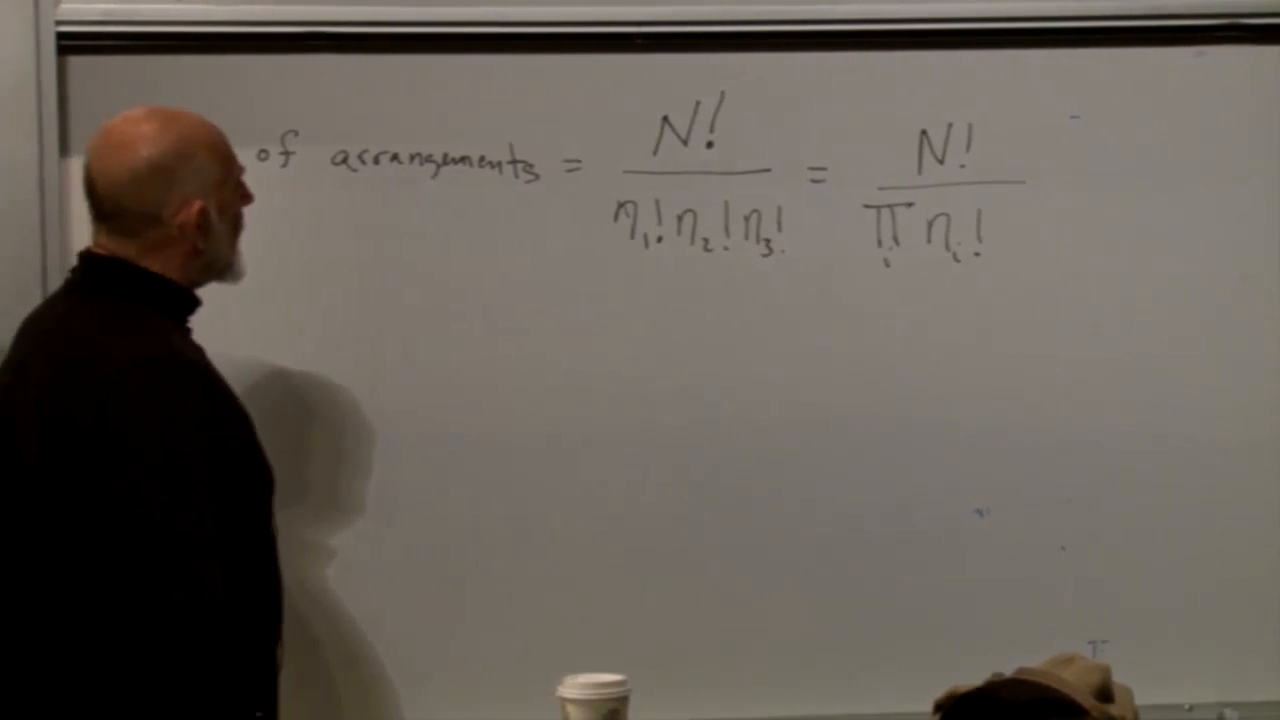
\includegraphics[width=0.88\textwidth]{lecture_03_figure_04.png}
\caption{黑板上写出的多项式 multiplicity
\(C=N!/\prod_i n_i!\)。}
\lectureframe{00:46:55}
\end{figure}

未被占据的能级不会造成问题，因为\(0!=1\)。如果所有复制品都占据一个态，那么
\[
 C=\frac{N!}{N!}=1,
\]
正如预期。如果三个复制品占据三个不同的指定态，那么
\[
 C=\frac{3!}{1!\,1!\,1!}=6.
\]
当两个复制品占据两个指定态时，该公式给出两种分配：交换哪个带标记的复制品占据哪个态。

\begin{classroomqa}
\audiencequestion{是否可能有不止一组占据数满足这两个约束条件？}
\lecturerresponse{通常有许多组都满足。方程
\eqref{eq:sm3-multiplicity}首先对某一固定组\(\{n_i\}\)计算排列数，此时尚未判定它是否满足约束条件。下一阶段则比较所有与约束相容的组，并找出其中 multiplicity 最大的那一组。
\lecturetimestamp{00:48:07--00:48:43}}
\end{classroomqa}

统计假设是：与孤立装置相容的微观分配被对称地对待。因此，由更多分配实现的一种宏观占据模式就更可能。对于大的\(N\)，关于分数\(n_i/N\)的分布会变得尖锐地集中。平衡分数就是在\eqref{eq:sm3-number-constraint}和
\eqref{eq:sm3-total-energy-constraint}的约束下使\(C\)最大的那些值。

\section{斯特林近似}

早在\(N\)达到宏观值之前，阶乘就已经变得极其巨大，因此我们改用它们的对数。从
\begin{equation}
 \log N!=\sum_{x=1}^{N}\log x.
 \label{eq:sm3-log-factorial-sum}
\end{equation}
开始。对于大的\(N\)，该和式可用\(\log x\)下方的面积来近似：
\begin{align}
 \log N!
 &\simeq\int_1^N\log x\,dx\\
 &=\left[x\log x-x\right]_1^N\\
 &=N\log N-N+1.
 \label{eq:sm3-stirling-integral}
\end{align}
原函数立即可由
\[
 \frac{d}{dx}(x\log x-x)=\log x.
\]
得到。在领先的广延阶下，可以略去加性常数：
\begin{equation}
 \log N!\simeq N\log N-N.
 \label{eq:sm3-stirling-log}
\end{equation}
取指数便得到讲座中所用的简化形式，
\begin{equation}
 N!\simeq N^N e^{-N}.
 \label{eq:sm3-stirling-simple}
\end{equation}

\begin{figure}[t]
\centering
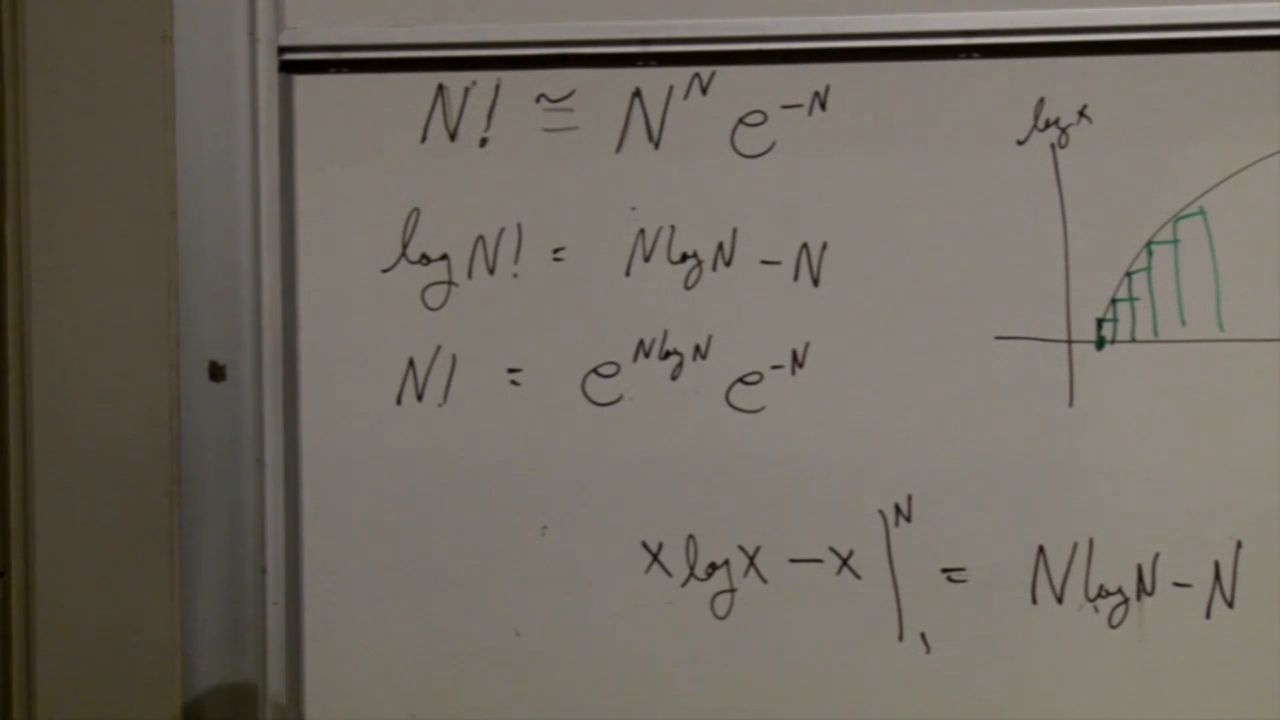
\includegraphics[width=0.88\textwidth]{lecture_03_figure_05.png}
\caption{领先的斯特林近似，以及通过将\(\log x\)的和式替换为积分而得到的推导。}
\lectureframe{01:03:45}
\end{figure}

\begin{classroomqa}
\audiencequestion{在下限处计算\(x\log x-x\)是否会留下一个额外的\(+1\)？}
\lecturerresponse{是的。方程\eqref{eq:sm3-stirling-integral}包含那个常数。当\(N\to\infty\)时，与正比于\(N\)的项相比，它可以忽略不计，这就是领先公式略去它的原因。和式本身必须从\(x=1\)开始；\(\log0\)没有定义。
\lecturetimestamp{01:04:12--01:04:35}}
\end{classroomqa}

\begin{classroomqa}
\audiencequestion{是否还缺少一个正比于\(\sqrt{N}\)的因子？}
\lecturerresponse{是的。更精确的渐近公式是
\[
 N!\sim\sqrt{2\pi N}\left(\frac{N}{e}\right)^N.
\]
它的对数只增加\(\tfrac12\log(2\pi N)\)，与\(N\log N-N\)相比是次广延的。它对于精确的有限\(N\)概率很重要，但对于宏观系统的领先熵计算并不重要。
\lecturetimestamp{01:04:35--01:05:40}}
\end{classroomqa}

在\eqref{eq:sm3-multiplicity}的分母中，也必须谨慎使用斯特林近似。在热力学极限下，具有非零极限概率的状态满足\(n_i=NP_i\)，因此它们的占据数随\(N\)增长。占据数极小或趋于零的状态可以通过有限能量截断来处理，然后再通过取极限恢复。被省略的次领头项不影响领头的广延熵。

\section{多重性的对数即熵}

对分子以及所有宏观上被占据的分母因子应用\eqref{eq:sm3-stirling-simple}：
\begin{equation}
 C\simeq
 \frac{N^Ne^{-N}}
 {\prod_i n_i^{\,n_i}e^{-n_i}}.
 \label{eq:sm3-c-stirling}
\end{equation}
由于\(\sum_i n_i=N\)，领头的指数因子相消：
\begin{equation}
 C\simeq\frac{N^N}{\prod_i n_i^{\,n_i}}.
 \label{eq:sm3-c-leading}
\end{equation}
对对数求极大比对乘积求极大更容易，而对数是单调的，所以两个极大值出现在同一占据模式上：
\begin{equation}
 \log C=N\log N-\sum_i n_i\log n_i.
 \label{eq:sm3-logc-occupations}
\end{equation}
现在代入\(n_i=NP_i\)：
\begin{align}
 \log C
 &=N\log N-\sum_iNP_i\log(NP_i)\\
 &=N\log N-N\sum_iP_i\log N
   -N\sum_iP_i\log P_i\\
 &=-N\sum_iP_i\log P_i,
 \label{eq:sm3-logc-entropy-derivation}
\end{align}
其中归一化使两个\(N\log N\)项相消。因此，在\(N\)的领头阶下，
\begin{equation}
 \boxed{\log C=NS}.
 \label{eq:sm3-logc-ns}
\end{equation}

\begin{figure}[t]
\centering
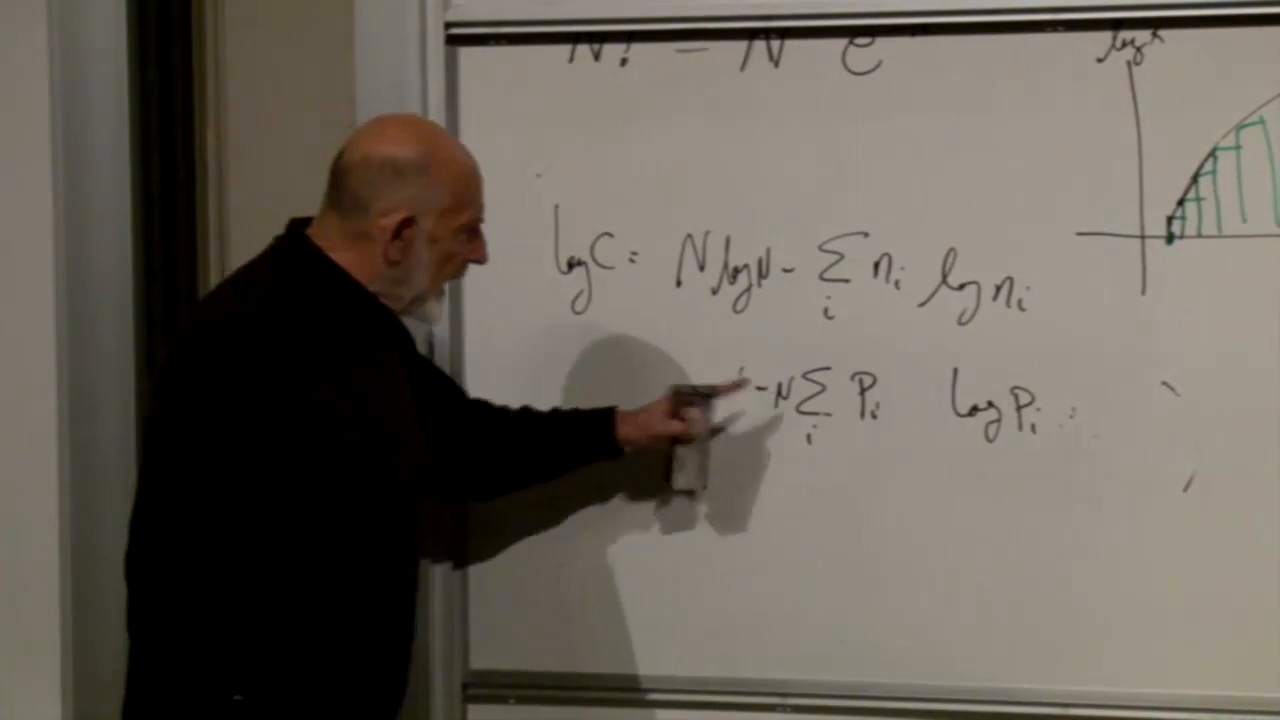
\includegraphics[width=0.88\textwidth]{lecture_03_figure_06.png}
\caption{将\(\log C=N\log N-\sum_i n_i\log n_i\)与\(-N\sum_iP_i\log P_i=NS\)联系起来的板书计算。}
\lectureframe{01:16:10}
\end{figure}

这一关系是本章的概念核心。熵并非强加于计数问题之上的一个无关量。它是每个复本的 multiplicity，以对数方式度量。因此，在领头阶下，最大化微观排列数等同于最大化一个复本的熵。

\begin{classroomqa}
\audiencequestion{当所有占据数都相等时，多重性难道不是最大吗？}
\lecturerresponse{当没有状态被区分，且只在一个有限状态集上施加\(\sum_i n_i=N\)时，它是均匀的。固定能量的约束改变了答案，因为\(E_i\)的值不同。相等的占据数一般无法产生指定的平均能量。
\lecturetimestamp{01:17:07--01:18:20}}
\end{classroomqa}

\begin{classroomqa}
\audiencequestion{大写\(N\)很大，但为什么可以对分母中的每一个\(n_i\)都应用斯特林近似？}
\lecturerresponse{对于每个具有非零极限概率的状态，\(n_i=NP_i\)正比于\(N\)增长。可以先保留一个有限能量范围，在其中取大\(N\)极限，然后再扩大该范围。稀疏的尾部状态需要单独的有限修正，但它们不改变领头的广延熵。
\lecturetimestamp{01:18:23--01:19:28}}
\end{classroomqa}

\begin{classroomqa}
\audiencequestion{这个大的\(N\)近似就是前面所说的粗粒化吗？}
\lecturerresponse{不是。热力学极限控制的是大占据数和渐近计数。粗粒化是微观分辨率的丢失或有意丢弃。它们是不同的操作，尽管在宏观统计力学中两者都经常被使用。
\lecturetimestamp{01:19:29--01:19:46}}
\end{classroomqa}

\begin{classroomqa}
\audiencequestion{既然\(\log C=N\log N-\sum_i n_i\log n_i\)，第二项难道不应该被最小化而不是最大化吗？}
\lecturerresponse{是的；在\(N\)固定的情况下，最大化\(\log C\)等价于最小化\(\sum_i n_i\log n_i\)。代入\(n_i=NP_i\)后，固定的\(N\log N\)项相消，剩下的就是\(-N\sum_iP_i\log P_i=NS\)。因此，同一操作更自然地描述为最大化正熵\(S\)。
\lecturetimestamp{01:19:48--01:20:55}}
\end{classroomqa}

\begin{classroomqa}
\audiencequestion{为什么不直接利用对称性令所有\(n_i\)相等，从而立即完成论证？}
\lecturerresponse{这种捷径忽略了能量标签。归一化约束对称地对待各状态，但\(\sum_iP_iE_i=\overline E\)并非如此：不同能量的状态贡献不同。能量约束正是非均匀平衡分布进入之处。
\lecturetimestamp{01:21:15--01:21:41}}
\end{classroomqa}

\section{最大熵问题}

现在我们可以毫无歧义地陈述统计力学规则。改变概率\(P_i\)并最大化
\begin{equation}
 S[P]=-\sum_iP_i\log P_i
 \label{eq:sm3-maximize-entropy}
\end{equation}
受约束于
\begin{equation}
 \sum_iP_i=1,
 \qquad
 \sum_iP_iE_i=\overline E.
 \label{eq:sm3-maxent-constraints}
\end{equation}
使该式最大的概率给出大复本系综中尖锐偏好的占据分数。占据数会涨落，但它们的相对偏差随\(N\)增大而缩小，因此比值\(n_i/N\)成为定义良好的热力学概率。

\begin{classroomqa}
\audiencequestion{\(E_i\)是固定的状态能量，而约束使用的是另外给定的总能量吗？}
\lecturerresponse{是的。谱\(\{E_i\}\)属于子系统。完整的复本集合具有固定的总能量，但能量不断在复本之间转移。将该总量除以\(N\)固定的是一个复本的平均能量\(\overline E\)，而不是它在每个微观实现中的能量。
\lecturetimestamp{01:26:12--01:27:07}}
\end{classroomqa}

这个问题容易陈述，但尚未解决。它是一个带有两个约束的极值问题，因此还需要一个数学工具。

\section{拉格朗日乘子}

对于无约束函数 \(F(x_1,x_2,\ldots)\)，驻点满足
\begin{equation}
 \frac{\partial F}{\partial x_i}=0
 \qquad\text{for every }i.
 \label{eq:sm3-unconstrained-stationary}
\end{equation}
现在再要求
\begin{equation}
 G(x_1,x_2,\ldots)=0.
 \label{eq:sm3-one-constraint}
\end{equation}

\begin{classroomqa}
\audiencequestion{如果图中坐标是 \(x\)
和 \(y\)，那么 \(x\) 是什么意思？}
\lecturerresponse{这里 \(x\) 是整个坐标向量
\((x_1,x_2,\ldots)\) 的简写。在二维图中，它的分量就是
\(x\) 和 \(y\)。之后这些分量将是概率
\(P_1,P_2,\ldots\)。
\lecturetimestamp{01:30:12--01:30:20}}
\end{classroomqa}

从几何上看，等值线 \(F=\text{constant}\) 构成一幅等高线图，
而 \(G=0\) 是系统被允许在其上运动的曲线。约束极值出现在
\(F\) 的某条等值线与约束曲线相切之处。在该点，梯度平行：
\begin{equation}
 \nabla F=-\lambda\nabla G
 \label{eq:sm3-parallel-gradients}
\end{equation}
其中 \(\lambda\) 是某个数。

\begin{figure}[t]
\centering
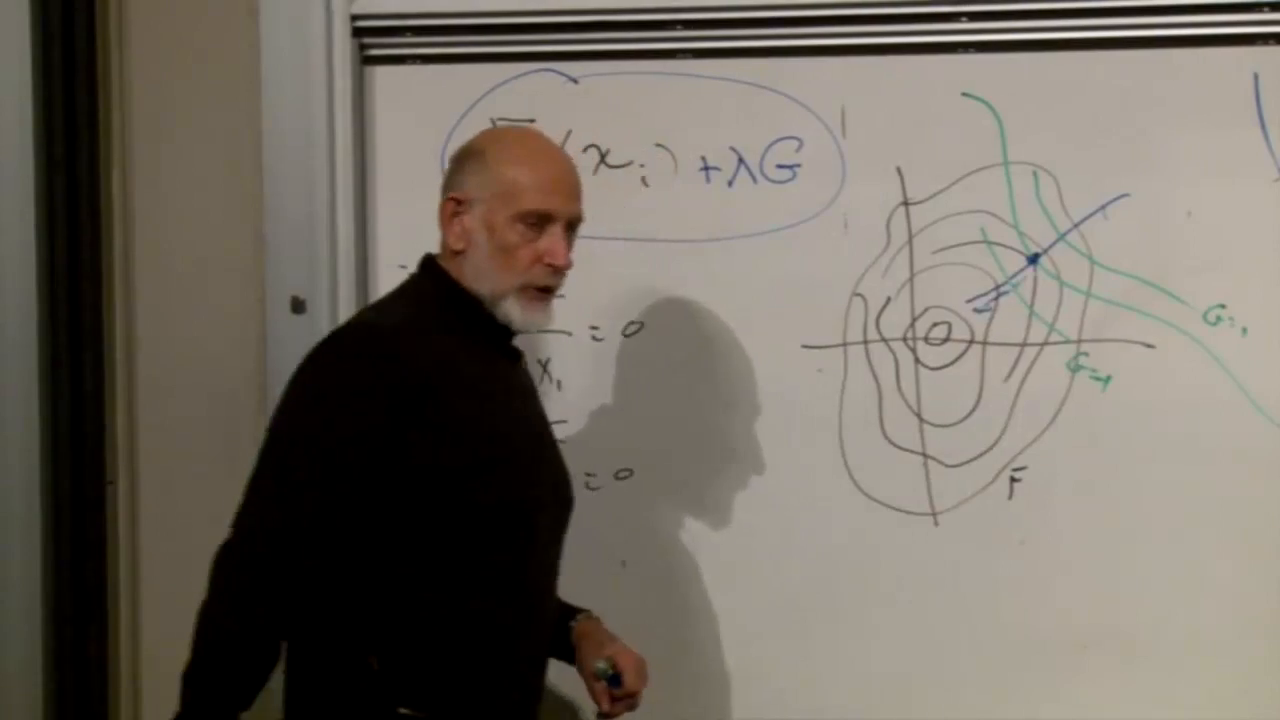
\includegraphics[width=0.88\textwidth]{lecture_03_figure_07.png}
\caption{黑板上的等高线几何以及增广函数
\(F'=F+\lambda G\)。约束极值出现在相切处。}
\lectureframe{01:37:10}
\end{figure}

方程 \eqref{eq:sm3-parallel-gradients} 可以通过定义
增广函数
\begin{equation}
 F'=F+\lambda G
 \label{eq:sm3-augmented-function}
\end{equation}
并要求普通驻点条件得到：
\begin{equation}
 \frac{\partial F'}{\partial x_i}=0.
 \label{eq:sm3-augmented-stationarity}
\end{equation}
乘子 \(\lambda\) 起初未知。这并不会使系统欠定，因为原约束 \(G=0\) 提供了一个
额外方程。

\begin{classroomqa}
\classquestion{为什么加上一个正比于 \(G\) 的项会使
约束点成为驻点？}
\lecturerresponse{在约束极值处，沿 \(G=0\) 的切向运动
已经不产生 \(F\) 的一阶变化。唯一剩余的斜率垂直于约束。由于 \(\nabla G\) 指向同一个法向，
适当的 \(\lambda\) 会将其抵消：
\(\nabla F+\lambda\nabla G=0\)。
\lecturetimestamp{01:35:06--01:35:32}}
\end{classroomqa}

\section{一个二变量例子}

最小化
\begin{equation}
 F(x,y)=\frac{x^2+y^2}{2}
 \label{eq:sm3-example-f}
\end{equation}
受约束于
\begin{equation}
 x+y=1.
 \label{eq:sm3-example-constraint}
\end{equation}
将约束写成 \(G=x+y-1=0\) 并构造
\begin{equation}
 F'=\frac{x^2+y^2}{2}+\lambda(x+y-1).
 \label{eq:sm3-example-augmented}
\end{equation}
驻点方程为
\begin{align}
 \frac{\partial F'}{\partial x}&=x+\lambda=0,\\
 \frac{\partial F'}{\partial y}&=y+\lambda=0.
 \label{eq:sm3-example-derivatives}
\end{align}
因此 \(x=y=-\lambda\)。剩下的方程就是约束，
\[
 x+y=-2\lambda=1,
\]
所以
\begin{equation}
 \lambda=-\frac12,
 \qquad
 x=y=\frac12.
 \label{eq:sm3-example-solution}
\end{equation}
点 \((1/2,1/2)\) 是以原点为圆心的最小圆与直线 \(x+y=1\) 相切之处。

\begin{figure}[t]
\centering
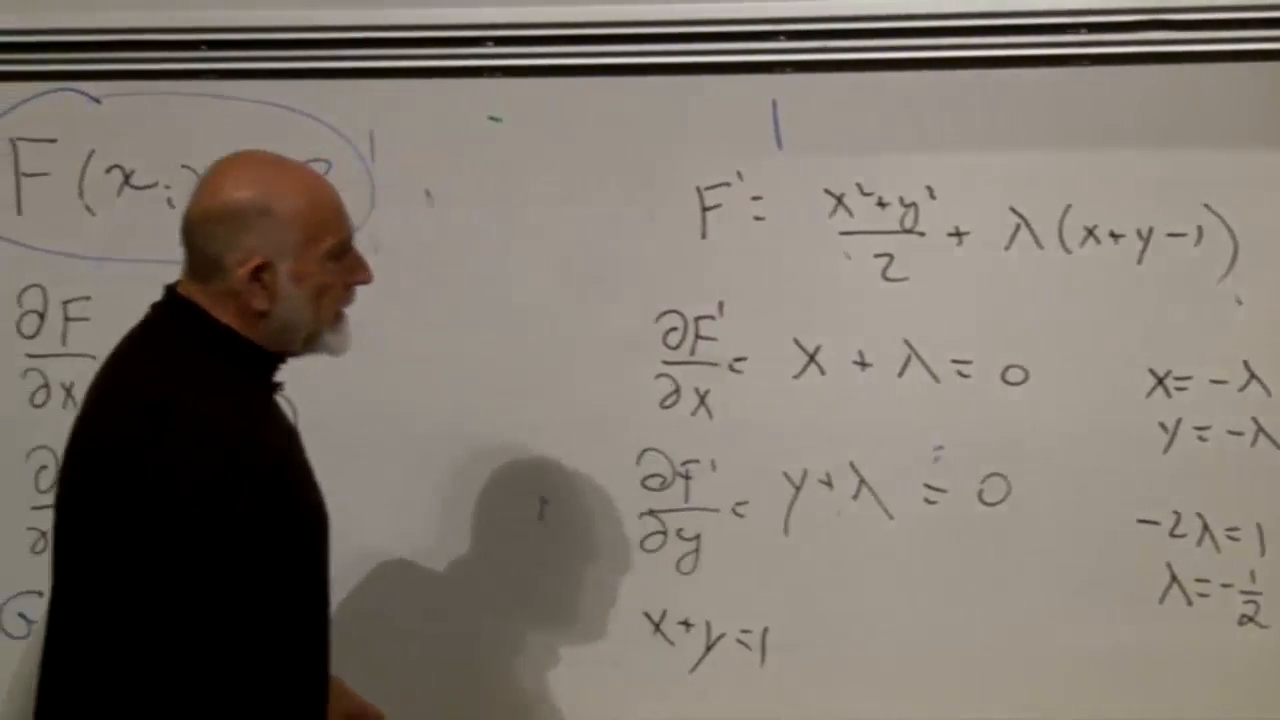
\includegraphics[width=0.88\textwidth]{lecture_03_figure_08.png}
\caption{为最小化 \((x^2+y^2)/2\) 且受约束于 \(x+y=1\) 而完成的拉格朗日乘子计算。}
\lectureframe{01:44:10}
\end{figure}

有多个约束时，为每个约束引入一个乘子：
\begin{equation}
 F'=F+\lambda_1G_1+\lambda_2G_2+\cdots.
 \label{eq:sm3-many-multipliers}
\end{equation}
然后求解
\begin{equation}
 \begin{aligned}
 \frac{\partial F'}{\partial x_i}&=0
 &&\text{for every }i,\\
 G_a&=0
 &&\text{for every constraint }a.
 \end{aligned}
 \label{eq:sm3-many-equations}
\end{equation}
本讲提出一个刻意人为的练习题：在施加两个独立线性约束（例如 \(x+y=1\) 和 \(z+x=1\)）的同时，求 \(x,y,z\) 的二次函数的极值。其目的不是那个具体答案，而是这条规则：每个约束都同时带来一个乘子和一个方程。

\section{为下一讲准备好的问题}

对于统计力学，坐标是概率
\(\{P_i\}\)，要最大化的函数是熵，约束是归一化和固定平均能量。定义
\begin{align}
 S[P]&=-\sum_iP_i\log P_i,\\
 G_1[P]&=\sum_iP_i-1,\\
 G_2[P]&=\sum_iP_iE_i-\overline E.
 \label{eq:sm3-final-functions}
\end{align}
因此增广熵可以写成
\begin{equation}
 \Phi[P]
 =S[P]+\alpha G_1[P]+\beta G_2[P].
 \label{eq:sm3-final-augmented}
\end{equation}
要求解的方程是
\begin{equation}
 \frac{\partial\Phi}{\partial P_i}=0
 \quad\text{for every }i,
 \qquad
 G_1=0,
 \qquad
 G_2=0.
 \label{eq:sm3-final-problem}
\end{equation}

\begin{figure}[H]
\centering
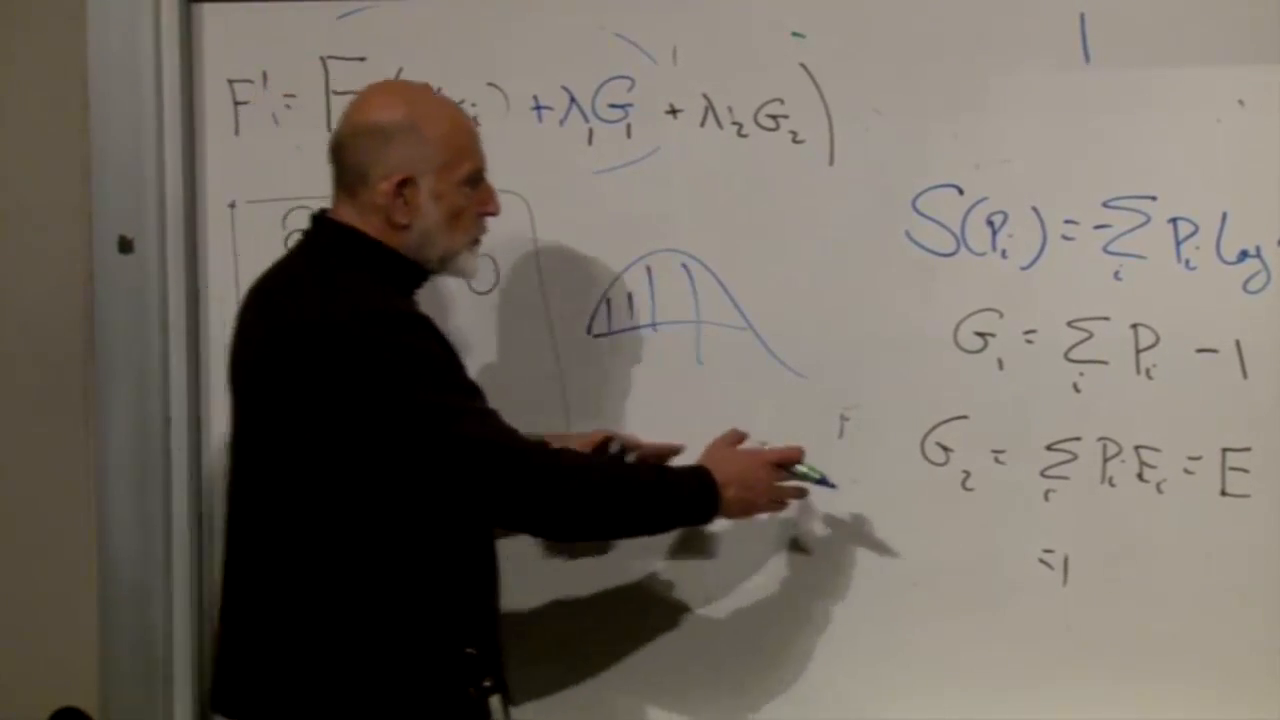
\includegraphics[width=0.88\textwidth]{lecture_03_figure_09.png}
\caption{收尾板书：作为概率函数的熵，连同归一化和固定平均能量。}
\lectureframe{01:53:05}
\end{figure}

至此，问题已经完全提出。求解
\eqref{eq:sm3-final-problem} 会给出平衡分布。与能量共轭的乘子将成为逆温度
\(\beta=1/T\)，具体取决于 \eqref{eq:sm3-final-augmented} 中所选的符号约定。下一讲将进行该微分运算并得到玻尔兹曼权重。
